\documentclass[12pt,fleqn]{article}

\title{A method for smoothing Impulse Response Functions for
  discrete-time linear models}

\author{Gray Calhoun\thanks{%
    Economics Department, Iowa State University;
    \protect\url{gcalhoun@iastate.edu},
    web: \protect\url{http://gray.clhn.org}.
    Helle Bunzel, Seth Pruitt, and participants in the ISU Statistical
    Graphics Working Group gave very helpful feedback on early
    versions of this paper.}}

% Check if shell commands can be executed
\ifnum\pdfshellescape=1
% Yes, enabled
\newcommand{\VERSION}{\splice{echo `git log -1 --date=short --format=\%cd`, `git describe --dirty`}}
\else
% No, disabled
\providecommand\VERSION{\today}
\fi
\date{\VERSION}
\usepackage{amsmath}
\usepackage{lucidabr}
\usepackage[margin=1in]{geometry}
\usepackage{
    amsfonts,
    amssymb,
    amsthm,
    bashful,
    bm,
    booktabs,
    enumitem,
    fancyhdr,
    flexisym,
    graphicx,
    mathtools,
    ragged2e,
    sectsty,
    setspace,
    slantsc,
    tabularx,
    tocstyle,
    url,
}
\allsectionsfont{\normalsize\RaggedRight}

\urlstyle{same}
\newcolumntype{C}{>{\centering\arraybackslash}X}

\pagestyle{fancy}
\renewcommand{\sectionmark}[1]{\markboth{}{\footnotesize{\thesection. #1}}}
\renewcommand{\subsectionmark}[1]{\markboth{}{\footnotesize{\thesubsection. #1}}}
\renewcommand{\headrulewidth}{0pt}
\renewcommand{\footrulewidth}{0pt}
\fancyhead[LE,LO]{\textit{\footnotesize{\nouppercase{\rightmark}}}}
\rhead{\footnotesize{\textit{\VERSION}}}

\onehalfspacing

\usepackage[small]{caption}
\usepackage[T1]{fontenc}
\usepackage[letterspace=35]{microtype}
\usepackage[sort,round,comma]{natbib}
\bibliographystyle{abbrvnat}
\newcommand\citepos[2][]{\citeauthor{#2}'s \citeyearpar[#1]{#2}}
\newcommand\poscw{\citeauthor{ClW:06}'s \citeyearpar{ClW:06,ClW:07}}
\newcommand\citen[1]{\citeauthor{#1}, \citeyear{#1}}

\newtheorem{proposition}{Proposition}

\renewcommand{\Re}{\operatorname{Re}}
\renewcommand{\Im}{\operatorname{Im}}

\DeclareMathOperator{\whitenoise}{\mathit{white\ noise}}
\DeclareMathOperator{\E}{E}
\DeclareMathOperator{\floor}{floor}
\DeclareMathOperator{\ceil}{ceil}

\newcommand{\vep}{\varepsilon}
\newcommand{\AR}{\allcaps{AR}}
\newcommand{\RR}{\mathbb{R}}
\newcommand{\VECM}{\allcaps{VECM}}

\newcommand{\Fs}{\mathcal{F}}

%%% Local Variables:
%%% mode: latex
%%% TeX-master: "../smoothirf.tex"
%%% TeX-command-extra-options: "-shell-escape"
%%% End:


\begin{document}
\maketitle
\begin{abstract}\noindent%
  We show how to construct continuous and differentiable Impulse
  Response Functions for discrete-time Vector Autoregressions and
  Vector Error-Correction Models. Current methods produce piecewise
  linear functions that introduce visual distortions, especially when
  many response functions are plotted in the same graph to represent
  uncertainty or partial identification. We also show how to plot the
  cumulative response to a shock and incorporate moving average
  dynamics.
\end{abstract}

\tableofcontents
\newpage

\section{Introduction}
\label{S1}

Impulse Response Functions (IRFs) are widely used in macroeconomics
to represent the dynamic effect over time of an unanticipated
shock. If $y_t$ is a stationary sequence of random vectors, an IRF
is a graph of the change in the conditional expectation of $y_{t+s}$
in response to an unanticipated shock to $y_t$, plotted as a function
of $s$. The conditional expectation may be implied by a theoretical
model or a statistical model, such as a VAR, in which case additional
assumptions may be necessary to identify the shocks of economic
interest. In either of these cases, IRFs can provide a parsimonious and
interpretable summary of the key features of the model.

Producing an IRF requires calculating the conditional expectation
$\E_t y_{t+s}$ under different counterfactual scenarios, with and
without the shock of interest. Since most macroeconomic models are
defined and estimated in discrete time (both $t$ and $s$ are integers)
the conditional expectations used to produce IRFs are calculated in
discrete time as well. (See Chapter 1 of \citealp{Ham:94}, for
example.) But in most applications, it is desirable to graph the IRFs
as curves and connect the points between the integer values of $s$;
this is especially important when more than one IRF is plotted on
the same graph --- whether to represent dynamics under different
assumptions (see \citealp{BeM:98}, and \citealp{StW:01}, for
representative examples), to represent statistical uncertainty
(\citealp{Kil:98}, and \citealp{SiZ:99}) or to represent regions that
are partially identified (\citealp{Uhl:05}, and
\citealp{InK:13}). Currently, this is done by linear interpolation
between the integer values of $\E_t y_{t+s}$ but this practice has
some drawbacks. Linear interpolation introduces misleading visual
distortions and can remove potentially interesting dynamics from the
model.

In this paper, we show how to construct continuous and smooth IRFs
for vector ARMA and other linear time series models. These IRFs are
defined for all values of $t$ and $s$, even noninteger values, and
ensure that the interpolation obeys the same dynamics as the rest of
the model. The resulting graph removes the distortions introduced by
current methods.  Section~\ref{S2} presents these results,
Section~\ref{S3} provides some numeric and empirical examples, and
Section~\ref{S4} concludes.

\section{Method for smoothing IRFs}
\label{S2}

This section presents the main results of the paper: smooth IRFs for
finite-order linear models. Section~\ref{S2.1} presents results for
the AR(1) to motivate our approach. Section~\ref{S2.2} extends this
result to finite-order VARs and Section~\ref{S2.3} extends the
result further to VARMA and VECM models and to cumulative responses.
The rest of this subsection introduces some notation and defines the
IRFs formally.

Let $\{y_t\}$ be a stationary sequence of random vectors in $\RR^k$,
let $\Fs_t$ represent the information set available in period $t$,
\begin{equation*}
  \Fs_t = \sigma(y_t, y_{t-1}, y_{t-2},\dots),
\end{equation*}
and let the function $m_s$ represent the conditional expectation of
$y_{t+s}$ given $y_t$, so
\begin{equation*}
  m_s(x) = \E(y_{t+s} \mid y_t = x)
\end{equation*}
for each $s \geq 0$. Define $m_s = 0$ for $s < 0$ and let
$\E y_t = \mu$. For a shock of interest $u$, with $u \in \RR^k$, the
IRF corresponding to $u$ is the function
\begin{equation}
  \label{eq:16}
  \Psi_{u}(s) = \E(m_s(y_t + u) - m_s(y_t)).
\end{equation}
The shock, $u$, in these equations should be viewed as the ``reduced
form'' version of the shock --- an unanticipated change in the current
value of $y_t$. In a Structural VAR application, $u$ will typically
be related to a more fundamental shock of economic interest $\delta$
through the linear transformation $u = \Gamma \delta$, for some known
or estimated matrix $\Gamma$.

If $y_t$ is nonstationary $\E_t$ may depend on the value of $t$. In that
case, define
\begin{equation*}
  m_{ts}(x_0,\dots,x_p)
  = \E(y_{t+s} \mid y_t = x_0,\dots, y_{t-p} = x_p)
\end{equation*}
and let
\begin{equation*}
  \Psi_{tu}(s) =
  m_{ts}(\E y_t + u, \E y_{t-1}, \dots, \E y_{t-p}) - m_{ts}(\E y_t, \E y_{t-1}, \dots,\E y_{t-p}).
\end{equation*}
Note that $\Psi_{tu}$ can be independent of $t$ even if $m_{ts}$ is
not.

\subsection{AR(1) motivation}
\label{S2.1}

\begin{figure}[t]
  \centering
  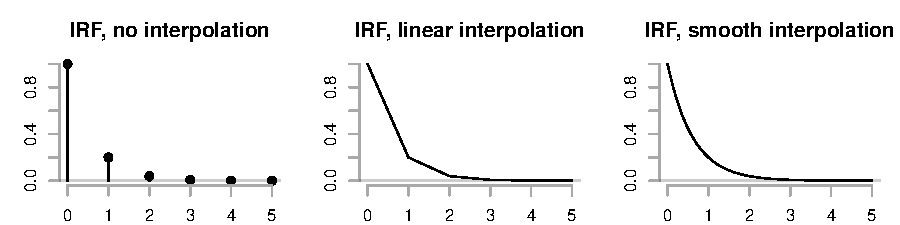
\includegraphics[width=6.5in]{graphs/motivation.pdf}
  \caption{IRF for simple AR(1) example. Here $y_t = 0.2 y_{t-1} +
    \vep_t$ --- the vertical axis shows $\Psi_1(s)$. The left panel
    plots only integer values of $s$, the middle panel uses linear
    interpolation between the integers, and the right panel plots the
    function $0.2^s$ directly.}
  \label{fig:1}
\end{figure}

For motivation, start with the simplest univariate case and assume
that $y_t$ is the AR(1)
\begin{equation}
  \label{eq:1}
  y_t = a y_{t-1} + \vep_t
\end{equation}
where $\vep_t$ is a martingale difference sequence and
$\lvert a \rvert < 1$.  For discrete-time models, it is easy to define
the IRF recursively and $\Psi_h(s) = a^s u$. When $a > 0$, this
function is well-defined for all positive real $s$, and can be used
directly to interpolate between the integer points. But typically
representing these dynamics has been achieved by linear interpolation,
so
\begin{align}
  \label{eq:2}
  \Psi_u(s)
  &= (s - \lfloor s\rfloor) \Psi_u(\lfloor s\rfloor+1)
    + (1 - s + \lfloor s\rfloor) \Psi_u(\lfloor s\rfloor) \\
  \label{eq:3}
  &= (s - \lfloor s\rfloor) a^{\lfloor s \rfloor + 1} u
    + (1 - s + \lfloor s\rfloor) a^{\lfloor s \rfloor} u
\end{align}
for noninteger $s$, where $\lfloor s\rfloor$ is the largest integer
less than or equal to $s$.

Figure~\ref{fig:1} plots $\Psi_u(s)$ for $u = 1$ and $a = 0.2$ using
three approaches: first only for the integer values of $s$, second
using linear interpolation between the integer values defined
by~\eqref{eq:3}, and finally using $a^s u$ directly for all
$s \geq 0$.\footnote{%
  All of the graphs in this paper were produced using R. \citep{R}} %
While one could debate which of the functions represents the `true'
impact of a shock at a fractional point in time and whether the
interpolated points should be interpreted, the dynamics and rate of
decay of the AR model are much more clearly represented by the right
panel that graphs $0.2^s$ directly.

This should not be surprising. We can see that $\Psi_u(s) = a^s u$
satisfies the recurrence relation implied by the lag structure of the
original AR process for any positive real value of $s$:
\begin{equation}
  \label{eq:4}
  \Psi_u(s) = a^s u = a \times a^{s-1} u = a \, \Psi_u(s-1).
\end{equation}
Letting $\Phi(L)$ define the lag polynomial of the AR(1) defined by
Equation~\eqref{eq:1}, (so the autoregressive model is defined as
$\Phi(L)y_t = \vep_t$ for all $t$) we can express~\eqref{eq:4} in a
form that will be easier to extend to more complicated DGPs,
\begin{equation}
  \label{eq:5}
  \Phi(L) \Psi_u(s) = (1 - a L) \Psi_{u}(s) = 0
\end{equation}
for all $s \in \RR^+$ with the implicit definition
$L \Psi_u(s) = \Psi_u(s-1)$. When $\Psi_u(s)$ is constructed by linear
interpolation, i.e.~\eqref{eq:3}, the recursive
relationships~\eqref{eq:4} and~\eqref{eq:5} only hold for integer
values of $s$.

\begin{figure}[t]
  \centering
  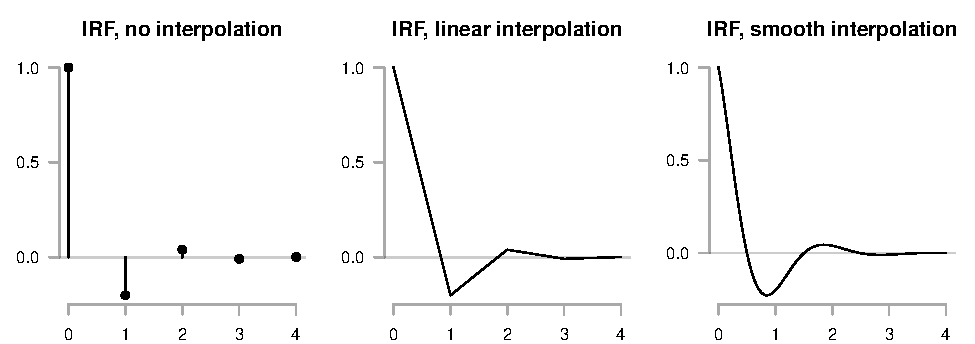
\includegraphics[width=6.5in]{graphs/motivation2.pdf}
  \caption{IRF for simple AR(1) example. Here $y_t = -0.2 y_{t-1} +
    \vep_t$ --- the vertical axis shows $\Psi_s(1)$. The left panel
    plots only integer values of $s$, the middle panel uses linear
    interpolation between the integers, and the right panel plots the
    function $|a|^s \cos(\pi s)$ directly.}
  \label{fig:2}
\end{figure}

The case $a \in (-1, 0)$ is slightly more complicated.  The previous
solution, $a^s u$, is well-defined and real-valued only for integer
values of $s$, so it can no longer be used directly for interpolation
between the noninteger points. Instead, consider the definition
\begin{equation}
  \label{eq:6}
  \Psi_u(s) = |a|^s \cos(\pi s) \cdot u.
\end{equation}
For integer values of $s$, $\cos(\pi s) = 1$ so~\eqref{eq:6} is
exactly equal to $a^s u$. But~\eqref{eq:6} remains real-valued and
well defined for noninteger $s$ as well. Moreover,~\eqref{eq:6}
satisfies the recurrence relation for the AR(1) model for all values
of $a \in (-1,1)$
\begin{equation*}
  \Psi_u(s) = |a|^s \cos(\pi s) \cdot u = - |a| \times |a|^{s-1} \cos(\pi (s-1)) \cdot u = a \, \Psi_u(s-1)
\end{equation*}
implying that
\begin{equation*}
  \Phi(L) \Psi_u(s) = (1 - a L) \, \Psi_u(s) = 0
\end{equation*}
as before. Figure~\ref{fig:2} plots the IRFs for $a = -0.2$ and
$u = 1$ with no interpolation, linear interpolation, and the
definition~\eqref{eq:6}. Just as before, the smooth version more
accurately reflects the system's dynamics after a shock.

This choice of $\Psi_u(s)$ was not made at random. Any complex
number $a + bi$ can be written in polar form,
\[
a + bi = R [\cos(\theta) - i \sin(\theta)]
\]
where $R = |a^2 + b^2|^{1/2}$ and $\theta$ satisfies
$\cos(\theta) = a/R$ and $\sin(\theta) = b/R$. Real powers of $a + bi$
can be expressed as\footnote{%
  See \citet{Ham:94} for background on complex numbers.} %
\[
(a + bi)^s = R^s [\cos(\theta s) - i \sin(\theta s)].
\]
For the AR example above, $a < 0$ and $b = 0$ so $\theta = \pi$.
Then $a^s = |a|^s \cos(\pi s)$ as we originally claimed.

This example also suggests a more general method for interpolating
between integer values of $s$ for any VAR; solve recurrence relation
using standard tools (as described in \citealp{Ham:94}, for example)
and use the solution as the IRF for real-valued $s$. We pursue that
approach in the next section.

\subsection{General Approach for VAR(\textit{p})}
\label{S2.2}

The AR(1) model in the previous section can be extended to general
VARs using the ``canonical'' representation.\footnote{%
  See \citet{Ham:94} or \citet{HaS:13} for a textbook treatment of
  much of this material. Our presentation borrows heavily from
  \citet{Ham:94}.} %
Define $y_t$ to be the VAR($p$),
\[
y_t = \sum_{j=1}^p A_j y_{t-j} + \vep_t.
\]
(We assume that $y_t$ has mean zero to simplify the presentation
without loss of generality.) To represent this relationship as a
VAR(1), form the vector $(y_t',\dots,y_{t-p+1}')'$ and observe
that
\begin{equation}
\label{eq:7}
\underbrace{\begin{pmatrix*}[l]
  y_t \\ y_{t-1} \\ y_{t-2} \\ \vdots \\ y_{t-p+1}
\end{pmatrix*}}_{Z_t}
=
\underbrace{\begin{pmatrix*}[l]
  A_1 & A_2 & \cdots & A_{p-1} & A_p \\
  I_k & 0   & \cdots & 0 & 0 \\
  0  & I_k  & \cdots & 0 & 0 \\
  \vdots & \vdots & \ddots & \vdots & \vdots \\
  0 & 0 & \cdots & I_k & 0
\end{pmatrix*}}_{F}
\underbrace{\begin{pmatrix*}[l]
  y_{t-1} \\ y_{t-2} \\ \vdots \\ y_{t-p+1} \\ y_{t-p}
\end{pmatrix*}}_{Z_{t-1}}
+
\underbrace{\begin{pmatrix*}[l]
  \vep_{t} \\ 0 \\ 0 \\ \vdots \\ 0
\end{pmatrix*}}_{U_t}.
\end{equation}
So this relationship is equivalent to $Z_t = F Z_{t-1} + U_t$. The
conditional expectation has a convenient form that is trivial to
calculate for integer values of $s$,
\begin{equation*}
  m_s(x) = e_{1p} F^s x
\end{equation*}
where $e_{jp}$ is the $k p \times k$ selection matrix
\begin{equation*}
  e_{jp} = \begin{pmatrix*}[l]
    0_{k \times (j-1)p} & I_k & 0_{k \times (k - j)p}
  \end{pmatrix*}.
\end{equation*}
Consequently, for integer values of $s$, the IRF has the form
\begin{equation*}
  \Psi_u(s) = e_{1p} F^s e_{1p}' u.
\end{equation*}
This section will argue that a variation of
this definition remains meaningful for noninteger values of $s$.

To show this, notice that, since $F$ is square, it has the Jordan
decomposition
\begin{equation}
  \label{eq:8}
  F = M J M^{-1}
\end{equation}

where $J$ is block diagonal of the form
\[
J = \begin{pmatrix*}[l]
  J_1 & \cdots & 0 \\
  \vdots & \ddots & \vdots \\
  0 & \cdots & J_q
\end{pmatrix*}
\]
and $q$ is the number of unique eigenvalues of $J_{\ell}$. Each
$J_\ell$ is an $n_\ell \times n_\ell$ matrix of the form
\[
J_\ell =
\begin{pmatrix*}[l]
  \lambda_\ell & 1 & 0 & \cdots & 0 & 0 \\
  0 & \lambda_\ell & 1 & \cdots & 0 & 0 \\
  0 & 0 & \lambda_\ell & \cdots & 0 & 0 \\
  \vdots & \vdots & \vdots & \ddots & \vdots & \vdots \\
  0 & 0 & 0 & \cdots & \lambda_\ell & 1 \\
  0 & 0 & 0 & \cdots & 0 & \lambda_\ell
\end{pmatrix*}
\]
where $\lambda_1,\dots,\lambda_q$ are the distinct eigenvalues of $F$
and $n_\ell$ is the number of times the $\ell$th eigenvalue is
repeated.  If all of the eigenvalues of $F$ are
distinct,~\eqref{eq:8} is just the eigenvalue decomposition of $F$.

This representation is convenient because, for positive integer values
of $s$, we have
\[
F^s = M J^s M^{-1}
\]
and
\begin{align*}
J^s =
\begin{pmatrix*}[l]
  J_1^s  & \cdots & 0      \\
  \vdots & \ddots & \vdots \\
  0      & \cdots & J_q^s
\end{pmatrix*}, &&
J_\ell^s &=
\begin{pmatrix*}[l]
  h_\ell(s,0) & h_\ell(s,1) & h_\ell(s,2) & \cdots & h_\ell(s,n_\ell)   \\
  0           & h_\ell(s,0) & h_\ell(s,1) & \cdots & h_\ell(s,n_\ell-1) \\
  0           & 0           & h_\ell(s,0) & \cdots & h_\ell(s,n_\ell-2) \\
  \vdots      & \vdots      & \vdots      & \ddots & \vdots             \\
  0           & 0           & 0           & \cdots & h_\ell(s,0)        \\
\end{pmatrix*},
\end{align*}
  where $h_\ell(s,j)$ is defined as
\begin{equation*}
h_\ell(s,j) =
\begin{cases}
  |\lambda_\ell|^s \big[\cos(\theta_\ell s) + i \sin(\theta_\ell s)\big] & j = 0 \\
  \frac{s!}{j!(s-j)!} |\lambda_\ell|^s \big[\cos(\theta_\ell s) + i \sin(\theta_\ell s)\big] & \text{if } s \geq j > 0 \\
  0 & \text{otherwise.}
\end{cases}
\end{equation*}
and $\theta_\ell$ satisfies
$\cos(\theta_\ell) = \Re(\lambda_\ell)/|\lambda_\ell|$ and
$\sin(\theta_\ell) = \Im(\lambda_\ell)/|\lambda_\ell|$ as before.

This representation allows us to write
\begin{multline}
  \label{eq:9}
  F^s =
  \sum_{j = 1}^q \sum_{l=0}^{\min(n_\ell, \lfloor s\rfloor)} \tfrac{s(s-1)\cdots(s-l+1)}{l (l - 1) \cdots 1} |\lambda_j|^{s-l} \\
  \times\Big\{\big[B_{jl} \cos(\theta_j s) + C_{jl} \sin(\theta_j s)\big] + i\big[D_{jl} \cos(\theta_j s) + E_{jl} \sin(\theta_j s)\big]\Big\}
\end{multline}
where the coefficient matrices $B_{jl}$, $C_{jl}$, $D_{jl}$, and
$E_{jl}$ are chosen to match $F^0, F^1, F^2,\dots$. For integer
values of $s$, the imaginary components of $M J^s M^{-1}$ exactly
cancel, so we can use the real part of~\eqref{eq:9} alone, giving
\begin{equation}
  \label{eq:10}
  F^s =
  \sum_{j = 1}^q \sum_{l=0}^{\min(n_\ell, \lfloor s \rfloor)} \tfrac{s(s-1)\cdots(s-l+1)}{l (l - 1) \cdots 1} |\lambda_j|^{s-l} \big[B_{jl} \cos(\theta_j s) + C_{jl} \sin(\theta_j s)\big]
\end{equation}
to produce $F^1, F^2, F^3,\dots$. Our proposal, in a nutshell, is to
use the definition given by~\eqref{eq:10} for all of the reals rather
than just the integers, exactly as we did in the motivating AR(1)
examples.

Equation~\eqref{eq:9} has another practical implication. Although
$F^s$ has real and imaginary components for real $s$, we are only
interested in its real component that generates the IRFs for integer
values of $s$. Rather than explicitly calculating the matrices
$B_{jl}$ and $C_{jl}$ to use~\eqref{eq:10}, we can calculate the
complex valued $F^s$ and simply drop its imaginary component. This
calculation is directly available in many programming languages and
can be implemented as $M J^s M^{-1}$ using the Jordan decomposition if
it is not.

We conclude this section with a formal statement of the result.

\begin{proposition}[Impulse Response Functions for VARs]
  \label{P1}
  Let $F$ be the coefficient matrix of the canonical VAR(1)
  representation of an arbitrary real-valued VAR($p$) $y_t$. Define
  $\Psi_{u}(s) = e_{1p} \Re(F^s) e_{1p}' u$ for all
  $s \in [0,+\infty)$, where $u \in \RR^k$ is a shock of theoretical
  interest. Then $\Psi_{u}(s)$ satisfies~\eqref{eq:16} for all
  integer values of $s$ and satisfies the recurrence relation implied
  by the original VAR for all positive, real values of $s$,
  \begin{equation}
    \label{eq:11}
    \Psi_u(s) = \sum_{j=1}^q A_j \Psi_u(s-j).
  \end{equation}
\end{proposition}
\begin{proof}
  The fact that $\Psi_u(s)$ meets the definition of the IRF on
  integers is discussed in the text and follows from simple
  algebra. Observe that the series $a_s = \Re(F^s) e_{1p}'u$ satisfies
  $a_s = F a_{s-1}$ since $F$ is real and
  \[
    F a_{s-1} = F \Re(F^{s-1}) e_{1p}'u
    = \Re(F^s) e_{1p}'u
    = a_s.
  \]
  The conclusion of this proposition is a direct consequence.
\end{proof}

\subsection[Finite-order linear models]{Extensions to other linear models}
\label{S2.3}

This section considers three extensions to the previous section.
First, we show how to calculate cumulative response functions for
VAR($p$)s. Second, we show how to calculate IRFs for Vector Error
Correction Models (VECM). And, third, we show how to calculate IRFs
for VARMA($p$, $q$) models. These results all rely on augmenting the
series to create a new canonical VAR(1) and can easily be combined
and extended further to other recursive linear models.

First, suppose that $y_t$ has a VAR($p$) representation as before.
but we want to derive the effect of the shock $u$ on $S_t$, the
cumulative sum of the $y_t$s,
\[
  S_t = \sum_{s=0}^t y_s.
\]
Since $S_t - y_t = S_{t-1}$, we can extend the canonical
representation for $y_t$ by embedding this relationship as the first
element of the vector $Z_t$ in~\eqref{eq:7}. Equation~\eqref{eq:7}
becomes
\begin{equation*}
  \begin{pmatrix*}[l]
    S_t - y_t \\ y_t \\ y_{t-1} \\ \vdots \\ y_{t-p+1}
  \end{pmatrix*}
  =
  \begin{pmatrix*}[l]
    I      & 0      & \cdots & 0       & 0      \\
    0      & A_1    & \cdots & A_{p-1} & A_p    \\
    0      & I      & \cdots & 0       & 0      \\
    \vdots & \vdots & \ddots & \vdots  & \vdots \\
    0      & 0      & \cdots & I       & 0
  \end{pmatrix*}
  \begin{pmatrix*}[l]
    S_{t-1}  \\ y_{t-1} \\ \vdots \\ y_{t-p+1} \\ y_{t-p}
  \end{pmatrix*}
  +
  \begin{pmatrix*}[l]
    0 \\ \vep_t \\ 0 \\ \vdots \\ 0
  \end{pmatrix*}
\end{equation*}
and can be rewritten as
\begin{equation*}
  \begin{pmatrix*}[l]
    S_t \\ y_t \\ y_{t-1} \\ \vdots \\ y_{t-p+1}
  \end{pmatrix*}
  =
  \underbrace{\begin{pmatrix*}[l]
    I      & A_1    & \cdots & A_{p-1} & A_p    \\
    0      & A_1    & \cdots & A_{p-1} & A_p    \\
    0      & I      & \cdots & 0       & 0      \\
    \vdots & \vdots & \ddots & \vdots  & \vdots \\
    0      & 0      & \cdots & I       & 0
  \end{pmatrix*}}_F
  \begin{pmatrix*}[l]
    S_{t-1}  \\ y_{t-1} \\ y_{t-2} \\ \vdots \\ y_{t-p}
  \end{pmatrix*}
  +
  \begin{pmatrix*}[l]
    \vep_t \\ \vep_t \\ 0 \\ \vdots \\ 0
  \end{pmatrix*}.
\end{equation*}
This representation is now a VAR(1) that can be handled exactly as in
Proposition~\ref{P1} and $\Psi_u(s)$ can be defined as
$e_{1,p+1} \Re(F^s) (e_{1,p+1} + e_{2,p+1})' u$

The VECM model has similar behavior. Suppose now that we have the
relationship
\begin{equation*}
  \Delta y_t = B y_{t-1} + A_1 \Delta y_{t-1} + \cdots + A_p \Delta
  y_{t-p} + \vep_t.
\end{equation*}
This can also be put in a canonical form using almost identical
arguments as before,
\begin{equation*}
  \begin{pmatrix*}[l]
    y_t \\ \Delta y_t \\ \Delta y_{t-1} \\ \vdots \\ \Delta y_{t-p+1}
  \end{pmatrix*}
  =
  \underbrace{\begin{pmatrix*}[l]
    (I + B) & A_1    & \cdots & A_{p-1} & A_p    \\
    B       & A_1    & \cdots & A_{p-1} & A_p    \\
    0       & I      & \cdots & 0       & 0      \\
    \vdots  & \vdots & \ddots & \vdots  & \vdots \\
    0       & 0      & \cdots & I       & 0
  \end{pmatrix*}}_F
  \begin{pmatrix*}[l]
    y_{t-1} \\ \Delta y_{t-1} \\ \vdots \\ \Delta y_{t-p+1} \\ \Delta y_{t-p}
  \end{pmatrix*}
  +
  \begin{pmatrix*}[l]
    \vep_t \\ \vep_t \\ 0 \\ \vdots \\ 0
  \end{pmatrix*}
\end{equation*}
and $\Psi_u(s)$ can be defined as
$e_{1,p+1} \Re(F^s) (e_{1,p+1} + e_{2,p+1})' u$ again.

VARMA($p$, $q$)s can also be handled similarly. If $y_t$ satisfies
\begin{equation*}
  y_t = \sum_{j=1}^p A_j y_{t-j} + \sum_{i=1}^q B_i \vep_{t-i} + \vep_t
\end{equation*}
this can be written as a canonical VAR(1) using the equation
\begin{equation*}
\begin{pmatrix*}[l]
  y_t \\ y_{t-1} \\ \vdots \\ y_{t-p+1} \\
  x_t \\ x_{t-1} \\ \vdots \\ x_{t-q+1}
\end{pmatrix*}
=
\underbrace{\begin{pmatrix*}[l]
  A_1    & \cdots & A_{p-1} & A_p    & B_1    & \cdots & B_{q-1} & B_q    \\
  I_k    & \cdots & 0       & 0      & 0      & \cdots & 0       & 0      \\
  \vdots & \ddots & \vdots  & \vdots & \vdots &        & \vdots  & \vdots \\
  0      & \cdots & I_k     & 0      & 0      & \cdots & 0       & 0      \\
  0      & \cdots & 0       & 0      & 0      & \cdots & 0       & 0      \\
  0      & \cdots & 0       & 0      & I_k    & \cdots & 0       & 0      \\
  \vdots &        & \vdots  & \vdots & \vdots & \ddots & \vdots  & 0      \\
  0      & \cdots & 0       & 0      & 0      & \cdots & I_k     & 0      \\
\end{pmatrix*}}_{F}
\begin{pmatrix*}[l]
  y_{t-1} \\ \vdots \\ y_{t-p+1} \\ y_{t-p} \\
  x_{t-1} \\ \vdots \\ x_{t-q+1} \\ x_{t-q}
\end{pmatrix*}
+
\begin{pmatrix*}[l]
  \vep_{t} \\ 0 \\ \vdots \\ 0 \\ \vep_t \\ 0 \\ \vdots \\ 0
\end{pmatrix*}.
\end{equation*}
Now $\Psi_u(s) = e_{1,p+q} \Re(F^s) (e_{1,p+q} + e_{p+1,p+q})' u$.

Other extensions are obviously also possible and these results can
be applied to state space models as well. See~\citet{HaS:13} for
additional examples and discussion.

\section{Examples}
\label{S3}
In this section, we present two examples. The first is a numerical
example that demonstrates how these methods scale when they are used
to graph many curves simultaneously. The second is an application to
Uhlig's~(2005) partial identification strategy for monetary policy
shocks.
\nocite{Uhl:05}

\subsection{Numerical example}
\label{S3.1}

For a simple numerical example, consider the two-variable VAR(2)
\begin{equation}
  \label{eq:12}
  \begin{pmatrix*}[l]
    y_{1t} \\ y_{2t}
  \end{pmatrix*}
  =
  \begin{pmatrix*}[r]
    - 0.50 & 0.01 \\ 0.30 & 0.10
  \end{pmatrix*}
  \begin{pmatrix*}[l]
    y_{1,t-1} \\ y_{2,t-1}
  \end{pmatrix*}
  +
  \begin{pmatrix*}[r]
    -0.20 & 0.10 \\ -0.10 & 0.00
  \end{pmatrix*}
  \begin{pmatrix*}[l]
    y_{1,t-2} \\ y_{2,t-2}
  \end{pmatrix*}
  +
  \begin{pmatrix*}[l]
    \vep_{1t} \\ \vep_{2t}
  \end{pmatrix*}
\end{equation}
and assume that $(\vep_{1t},\vep_{2t}) \sim N(0,I)$ represents the
shocks of interest.

The IRF for an $\vep_1$-shock is defined as described above,
\begin{equation*}
  \Psi_1(s) = e_{1,2} \Re(F^s) e_{1,2}'
  \begin{pmatrix*}[l]
    1 \\ 0
  \end{pmatrix*}
\end{equation*}
with
\begin{equation*}
F = \begin{pmatrix*}[r]
    - 0.50 & 0.01 & -0.20 & 0.10 \\
      0.30 & 0.10 & -0.10 & 0.00 \\
      1.00 & 0.00 & 0.00 & 0.00 \\
      0.00 & 1.00 & 0.00 & 0.00
  \end{pmatrix*}
\end{equation*}
Similarly, the IRF for an $\vep_2$-shock is given by
\begin{equation*}
  \Psi_2(s) = e_{1,2} \Re(F^s) e_{1,2}'
  \begin{pmatrix*}[l]
    0 \\ 1
  \end{pmatrix*}.
\end{equation*}

We plot the IRFs in the first two columns Figure~\ref{fig:3}. The
first column plots the standard IRFs, using linear interpolation
between integer-valued time periods, and the second plots our proposed
smooth plots. Although the general impressions from both graphs are
similar, there are important differences. First, peaks and troughs are
often underestimated by the standard IRFs and their timing is
frequently misidentified. This is especially apparent in the first
peak in the second row, which falls exactly on period $t+1$ using
linear interpolation but approximately $t+0.5$ using ours.  Second,
even the sign of the IRF can be misidentified, as we see with the
immediate response of $y_{1}$ to a shock in $\vep_{2}$.

However, it would be reasonable for researchers to want to emphasize
the value of the IRF at the integer time-periods, since those do not
depend on any method of interpolation. The third column of
Figure~\ref{fig:3} demonstrates one method of doing this: plot the
individual points of the IRF defined on the integers over a light
version of the curve.

\begin{figure}[t]
  \centering
  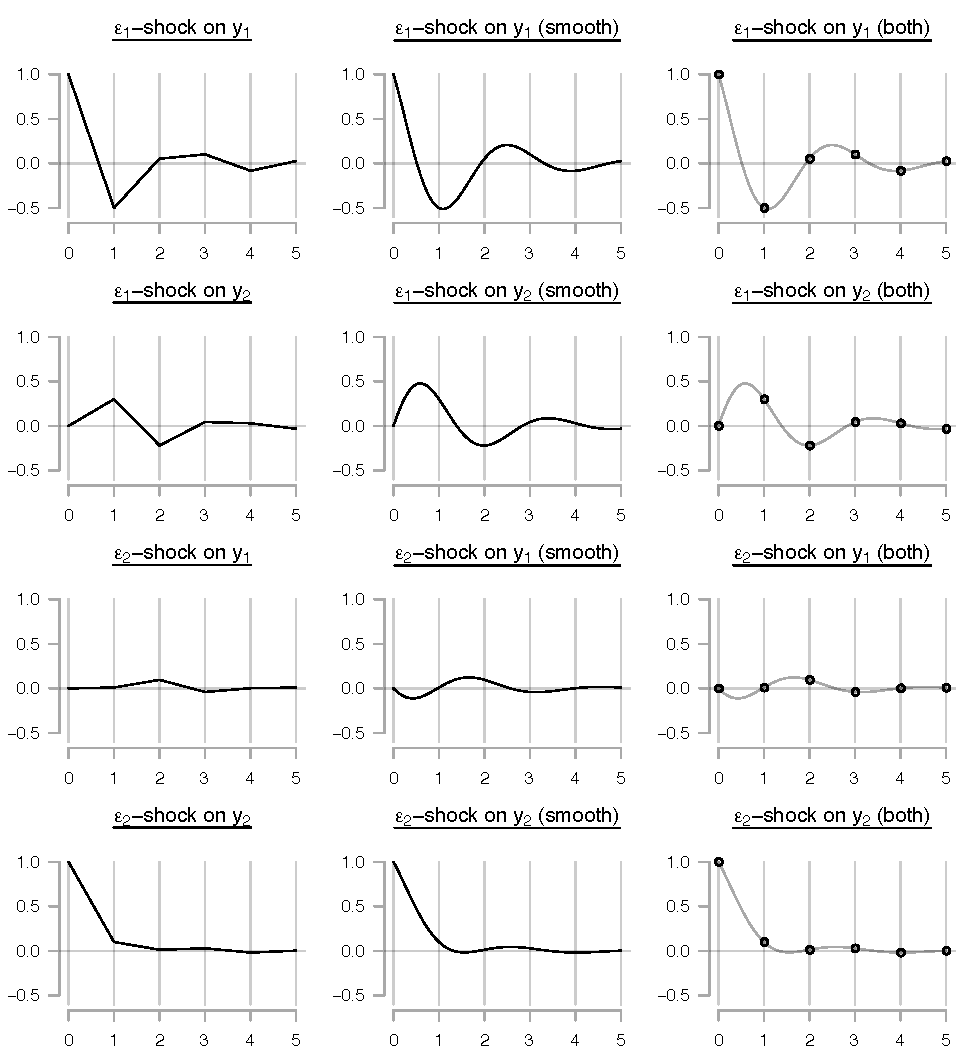
\includegraphics[width=6.5in]{graphs/numeric.pdf}
  \caption{Impulse Response Functions from Section~\ref{S3.1} example;
    $y_t$ is generated by Equation~\eqref{eq:12}. The left column
    plots standard IRFs, the middle column plots our new method, and
    the right column plots our new approach, emphasizing the values at
    integer time periods.}
  \label{fig:3}
\end{figure}

The weaknesses of using linear interpolation become more apparent when
we graph multiple perturbations of the IRFs in the same panel, which
is a common way of representing uncertainty or set-identified
responses. To demonstrate this phenomenon, we generated 150
perturbations of the IRFs by adding independent $N(0, 0.15)$ noise
terms to each element of the VAR coefficients in~\eqref{eq:12}, then
calculating and plotting the IRFs as before. (The graphs use alpha
blending, a form of partial transparency, to make the individual
curves more visible.)

\begin{figure}[t]
  \centering
  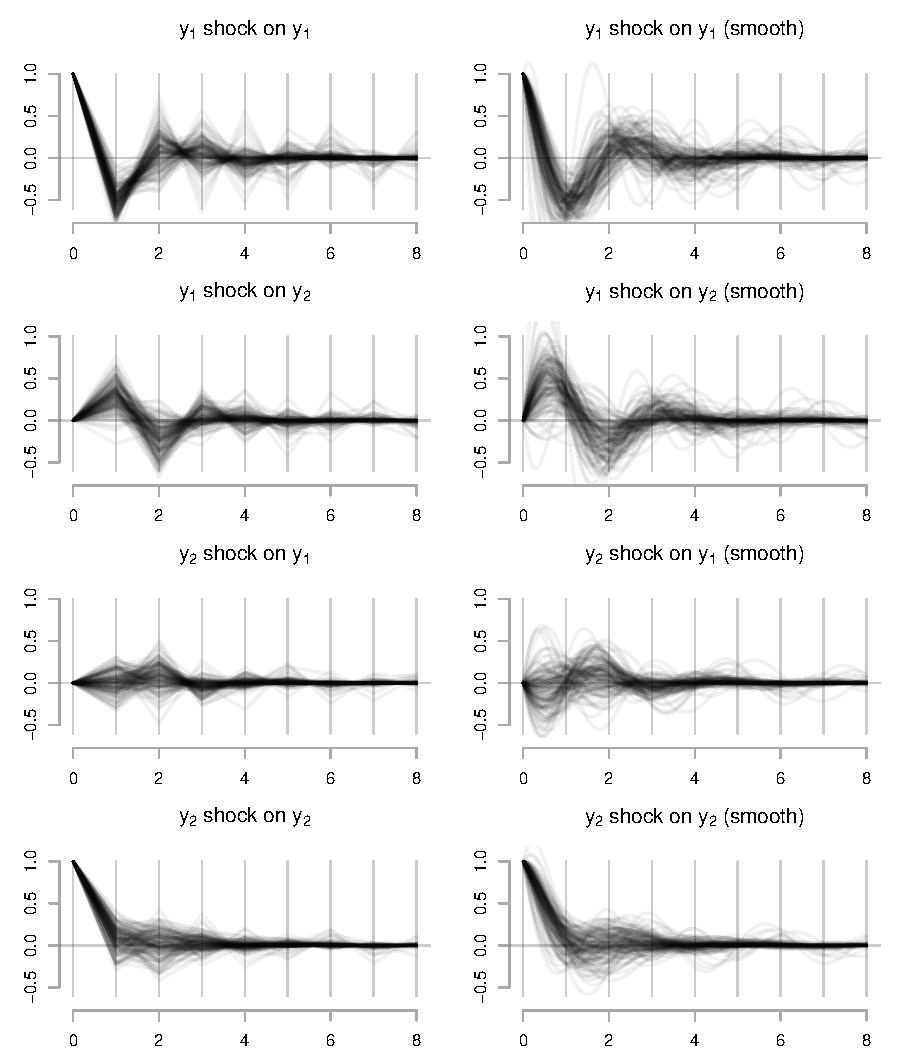
\includegraphics[width=6.5in]{graphs/numeric2.pdf}
  \caption{Impulse Response Functions from Section~\ref{S3.1} example;
    $y_t$ is generated by Equation~\eqref{eq:12} with independent
    $N(0,0.15)$ random variable added to each coefficient. These
    graphs plot the IRFs from 150 independent draws of the
    coefficient matrices. The left column plots standard IRFs, the
    middle column plots our new method, and the right column plots our
    new approach with an emphasis on the integer time periods..}
  \label{fig:4}
\end{figure}

These graphs are shown in Figure~\ref{fig:4}. The same issues apparent
in Figure~\ref{fig:3} are present here as well. But there are other
problems as well. In the first curve, for example, the discrete IRF
shows substantial negative correlation between the period 2 and period
3 estimated response and the period 3 and 4 response to an
$\vep_1$-shock. But the smoothed graph makes it clear that this is
driven by the timing and size of the first peak. When that peak is
near period 2, the curve has time to fall noticeably before period 2,
but when the peak is closer to period 3, the curve is still rising for
that interval. The actual dynamics implied by the different curves are
very similar. Similar but less dramatic distortions appear in the
other panels as well. In the third row, for example, the discrete
IRF shows that about half of the parameter values have an initial
increase in response to a $y_{20}$ shock and half have an initial
decrease, but the smooth curves show that virtually all of them have
an immediate decrease, but that many start to increase very soon. The
exact location of the peak that falls between periods 1 and 2
determines most of the initial dynamics, but this is impossible to see
in the discrete curve.

These graphs reveal that our method of constructing IRFs is more
resilient to perturbation than linear interpolation: curves generated
by close coefficient values have a more similar appearance. This
property is particularly useful when graphing many similar curves to
represent statistical uncertainty. Moreover, as the right columns in
Figures~\ref{fig:3} and~\ref{fig:4} illustrate, it is still possible
to emphasize the integer-valued time periods while using our method of
interpolation.

\subsection{Empirical analysis of the effect of monetary policy}
\label{S3.2}

This section demonstrates our proposed method for constructing IRFs
in a widely-studied empirical setting. We conduct a brief analysis of
the effect of monetary policy on the real economy using Uhlig's~(2005)
sign-restriction partial identification strategy.

First, a quick review. In Structural VAR models, the shocks of
theoretical interest --- a monetary policy shock in this section ---
can simultaneously affect all of the variables in the model. Without
additional assumptions beyond those necessary to estimate the
coefficients of the VAR, we can not estimate all of the unknown
parameters necessary to identify the shock.\footnote{%
  \citet{Kil:13} gives a recent review of the SVAR literature.} %
I.e., if $y_t$ is a VAR($p$),
\begin{equation}
  \label{eq:13}
  y_t = \alpha + \sum_{i=1}^p A_i y_{t-p} + \vep_t,
\end{equation}
with $\vep_t \sim (0, \Sigma)$ a martingale difference sequence, then
$\vep_t$ is related to the sequence of theoretical shocks $\delta_t$
through
\begin{equation*}
  \vep_t = \Gamma \delta_t
\end{equation*}
and $\delta_t \sim (0, I)$ is also martingale difference sequence. The
variance covariance matrix, $\Sigma$, can be consistently estimated,
but $\Gamma$ will in general have more unique elements than $\Sigma$.
The IRF corresponding to a vector of theoretical shocks $\delta$ is
given by
\begin{equation}
  \label{eq:14}
  \Psi_\delta(s) = e_{1p} \Re(F^s) e_{1p}' \Gamma \delta
\end{equation}
so additional restrictions on $\Gamma$ are necessary to estimate
$\Psi_\delta$.

\citet{Uhl:05} proposes using a minimal set of assumptions to identify
\emph{potential} monetary policy shocks. Letting the first element of
$\delta$ represent a positive monetary policy shock, Uhlig's approach
is to generate candidate shocks randomly and calculate $\Psi_\delta$
corresponding to that specific shock. IRFs that match some a priori
plausible criteria are kept as potential responses to monetary policy
shocks and the resulting set of functions partially identifies the
effect of a shock. Formally, for given estimates $\hat F$ and
$\hat \Sigma$, this procedure amounts to generating many candidate
shocks $u^* = u / \| u \|_2$ where $u \sim N(0,I)$ and calculating the
candidate IRFs as
\begin{equation}
  \label{eq:15}
  \hat \Psi_{u^*}(s) =  e_{1p} \Re(\hat F^s) e_{1p}' \hat\Sigma^{1/2} u^*,
\end{equation}
then discarding $\hat\Psi_{u^*}(s)$ that do not meet a set of criteria of
that define and constrain the monetary policy shock.

In this paper, we use our proposed method for graphing IRFs to plot
the candidate responses to a monetary policy shock using Uhlig's sign
restrictions. We fit a 6-lag VAR using the same six variables as
Uhlig: real GDP, the GDP deflator, the federal funds rate, borrowed
reserves, nonborrowed reserves, and a commodity price
index.\footnote{%
  As in Uhlig, we fit the model in levels and without an explicit time
  trend.} %
We also impose the same restrictions as Uhlig:
\begin{itemize}[noitemsep]
\item the Federal Funds rate does not increase for five months after a
  monetary policy shock,
\item the price level does not decrease for five months after a
  monetary policy shock, and
\item nonborrowed reserves does not decrease after a monetary policy
  shock.
\end{itemize}
Since our interest here is in the method of displaying IRFs, we use
\citeauthor{BeM:98}'s original dataset, which covers January 1965
through December 1997.  Most of the variables are available
monthly. Since GDP and the GDP deflator are only quarterly, their
values are interpolated as described by \citet{BGW:97} and
\citet{BeM:98} and we fit a VAR on the monthly data.

Figure~\ref{fig:5} presents our graphs.\footnote{%
  As in our earlier example, these graphs use partial transparency,
  alpha blending, to show as many of the individual curves as
  possible.} %
For this exercise, we only present the estimate of the identified set
that is associated with the OLS point estimates and ignore the
additional uncertainty in estimating the coefficients. The main
results are essentially already known: the immediate effect of a
sign-identified monetary policy shock on GDP is ambiguous in the very
short run but lowers GDP relative to trend after about two years. And
the effects on the other variables are consistent with the
identification strategy and with the previous literature. But our
approach to smoothing the IRFS allows each of the individual candidate
shocks to be studied as well. Many of the curves have a minimum
between 1/2 to 2 years, but there is considerable uncertainty over the
exact date of the minimum.  The dynamics expressed by the outer
envelope of the curves, which is the quantity plotted in many VAR
applications, is not particularly representative of any of the
individual IRFs.

\begin{figure}[t]
  \centering
  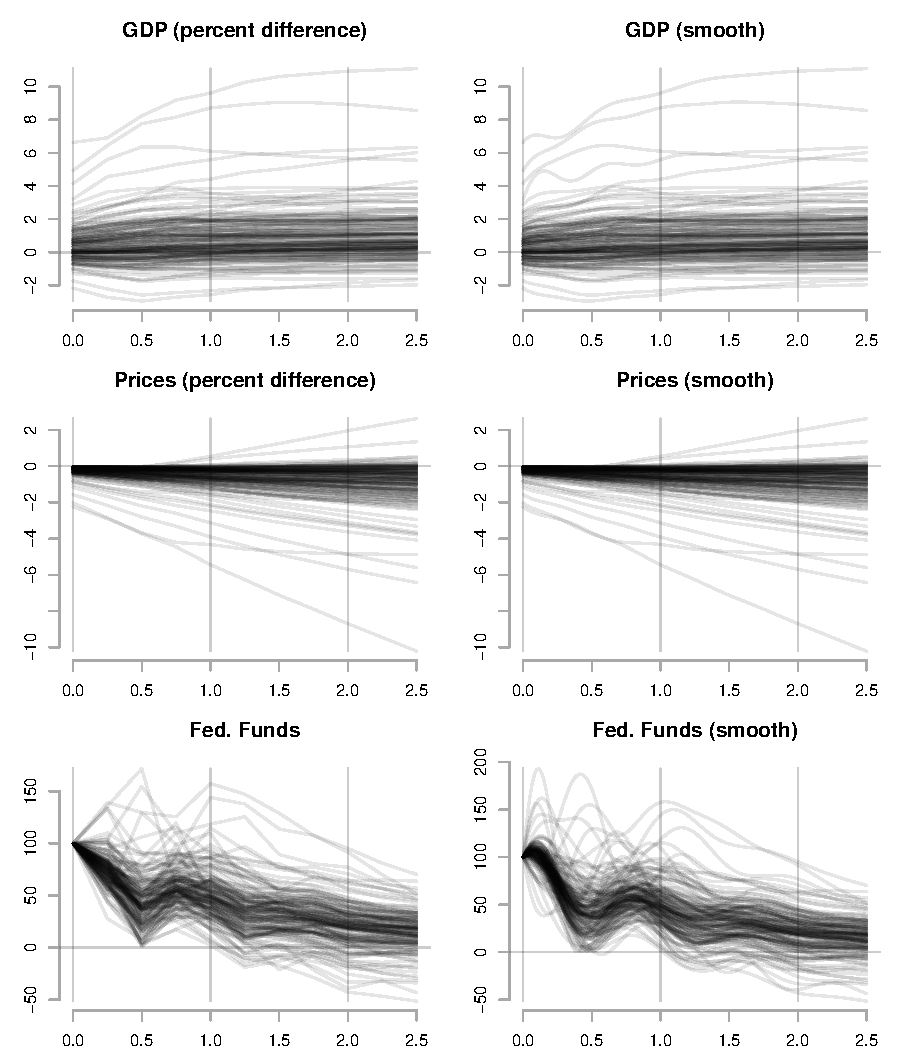
\includegraphics[width=6.5in]{graphs/empirics}
  \caption{%
    Empirical response of each variable to a sign-identified negative
    monetary policy shock; see description in Section~\ref{S3.2}. The
    horizontal axis is the number of years since the initial
    shock. These figures graph 500 candidate shocks.}
  \label{fig:5}
\end{figure}

\section{Conclusion}
\label{S4}

Vector Autoregressive models do not just have implications for the
period-to-period dynamics of a stochastic process, they also have
implications about the very short-run dynamics within periods. In this
paper, we propose that researchers graph those intra-period dynamics
when plotting the IRFs for linear models and we give a simple method
to do so, based on the model's canonical VAR(1) representation. Even
when researchers do not want to assign any economic importance to
these ultra short-run dynamics, plotting them in the IRFs minimizes
visual distortions that can arise from discretizing the dynamics,
especially when several IRFs are plotted over each other to
represent uncertainty or partial identification.

\clearpage
\addcontentsline{toc}{section}{References}
\bibliography{latex_misc/references}

\clearpage
\appendix
\section{Appendix: Changes to this paper from previous versions}
\begin{description}
\item{Latest:}
  \begin{itemize}[noitemsep]
  \item Rerender pictures to fix display problems in some pdf vieweres.
  \end{itemize}

\item{v0.3, 2016-03-28:}
  \begin{itemize}[noitemsep]
  \item Makes small wording changes to the abstract.
  \item Changes the title of the paper.
  \item Adds empirical analysis of monetary policy (as in Uhlig, 2005).
  \item Adds Git commit information to the pdf.
  \item Adds this changelog to the pdf.
  \item Adds a table of contents to the pdf.
  \item Makes several small formatting changes.
  \item Makes several small changes to the internal file organization.
  \end{itemize}

\item{v0.2.2, 2015-02-22:} Tweaks the abstract.

\item{v0.2.1, 2015-02-21:} Adds author affiliation.

\item{v0.2.0, 2015-02-21:} Adds cumulative response function and VECM section; and
  revises the text of the paper.

\item{v0.1.0, 2015-02-11:} First draft of the paper.
\end{description}

%%% Local Variables:
%%% mode: latex
%%% TeX-master: "smoothirf.tex"
%%% TeX-command-extra-options: "-shell-escape"
%%% End:

\end{document}

%%% Local Variables:
%%% mode: latex
%%% TeX-master: t
%%% TeX-command-extra-options: "-shell-escape"
%%% End:
